
%(BEGIN_QUESTION)
% Copyright 2014, Tony R. Kuphaldt, released under the Creative Commons Attribution License (v 1.0)
% This means you may do almost anything with this work of mine, so long as you give me proper credit

A FOUNDATION Fieldbus transmitter senses the level of fluid inside a fuel storage tank.  The operators need to see the volume of fuel stored inside the tank in units of {\it cubic feet}, while the level transmitter directly senses fuel level over a range of 0 to 5 feet.  The other dimensions of the tank are 12 feet by 6 feet.  Determine the proper {\tt L\_type}, {\tt XD\_Scale}, and {\tt OUT\_Scale} values to enter into this transmitter's Analog Input function block when configuring the system:

$$\includegraphics[width=15.5cm]{i03000x01.eps}$$

\underbar{file i03000}
%(END_QUESTION)





%(BEGIN_ANSWER)

\begin{itemize}
\item{} {\tt L\_type} = Indirect
\item{} {\tt XD\_Scale} = 0 to 5 feet
\item{} {\tt OUT\_Scale} = 0 to 360 cubic feet
\end{itemize}

%(END_ANSWER)





%(BEGIN_NOTES)

{\bf This question is intended for exams only and not worksheets!}.

%(END_NOTES)


